\documentclass[]{report}

% PREAMBLE

% A file like this(called home.tex) could be placed in each latex project folder. 

% This will give the possibility to use modules like this:
% % A file like this(called home.tex) could be placed in each latex project folder. 

% This will give the possibility to use modules like this:
% \input{home} - This is needed to use the \home command
% \input{\home/Modules/Usepackages}
% \input{\home/Modules/ChapterStyle}
% \input{\home/Modules/HeaderAndFooter}

% If you use Github or any other collaborating tool, you should ignore the home.tex file, so that every user could have their own home.tex file.

\newcommand{\home}{C:/Users/Kasper/Documents/GitHub/Latex} - This is needed to use the \home command
% \input{\home/Modules/Usepackages}
% \input{\home/Modules/ChapterStyle}
% \input{\home/Modules/HeaderAndFooter}

% If you use Github or any other collaborating tool, you should ignore the home.tex file, so that every user could have their own home.tex file.

\newcommand{\home}{C:/Users/Kasper/Documents/GitHub/Latex}
\input{\home/Modules/Usepackages}
\input{\home/Modules/ChapterStyle}
\input{\home/Modules/HeaderAndFooter}
\input{\home/Modules/Paragraph}
\input{\home/Modules/Figure}

% Put into module
\usepackage{bm}
\DeclareMathOperator*{\argmin}{arg\,min}
\DeclareMathOperator*{\argmax}{arg\,max}




%FixMe pakken viser små kommentarer, hvor der skal rettes
%--------------------------------------------------
%Brug med følgende: \fxnote{det her skal uddybes!} 
%Se liste over alle fixMe's: \listoffixmes
%Erstat 'draft' med 'final' for at fjerne alle kommentarer
%--------------------------------------------------
\usepackage[footnote,draft,english,silent,nomargin]{fixme}

% Title Page
\title{TiNONS Project - Speaker Recognition: Appendix}
\author{Kasper Nielsen - 10731 \\ Alexander Rasborg Knudsen - 20107083}



\begin{document}
\maketitle

\listoffixmes
\newpage

\tableofcontents


\chapter{Dataset}
\section{Description}
The data that we use to test individual classification methods in this project consists of recordings from 4 speakers repeatedly saying the numbers 0 through nine.
From this set one speaker was removed, because significantly fewer recordings ware made of this.
Hence the amount of data points less fewer than was desired.

Out of the dataset, 15 utterings of each digit ware selected randomly from each speaker, classified and put into the training set.
Another 5 utterings of each digit from each speaker was then classified ad selected as test set.

The data is sampled at $ 48\ kHz, 16\frac{bits}{sample}  $

The data is provided by \cite{DataSet}

\input{features_app} - DONE ?

% Evaluation method
\chapter{Evaluation of classification methods}
The individual classification methods are evaluated with datasets of varying complexities.
Most notably, with speakers uttering the same single digit ("\textit{ZERO}"), two different digits ("\textit{ZERO}" and "\textit{ONE}"), and ten different digits ("\textit{ZERO}", "\textit{ONE}" through "\textit{NINE}").


To evaluate a classifier, the confusion matrix is an ideal way of doing so.
The confusion matrix can show the classifications sensitivity, precision and accuracy for each class. 
The terms used to describe this is: false positive (\textit{FP}), true positive (\textit{TP}), false negative (\textit{FN}) and true negative (\textit{TN}).
The true terms are classes that are correctly classified and false terms are incorrectly classified.
The sensitivity is the probability of classifying the inputs as class $X$ for a input that are class $X$.
\begin{equation}
\mathtt{sensitivity}(X) = \dfrac{TP_X}{TP_X+\Sigma FN_X}
\label{eq:sensitivity}
\end{equation}
The precision is the probability that the estimate of class $X$ is correct.
\begin{equation}
\mathtt{precision}(X) = \dfrac{TP_X}{TP_X+\Sigma FP_X}
\label{eq:precision}
\end{equation}
The accuracy is the probability that the classification of any given class is correct, where N = total number of tests.
\begin{equation}
\mathtt{accuray}(X) = \dfrac{\Sigma TP_X}{\mathrm{N}}
\label{eq:accuracy}
\end{equation}

\begin{table}[H]                                              
\centering                                                     
\begin{tabular}{|l|c|c|c|c|}                                   
\hline                                                         
  & Speaker Jacob & Speaker Mose & Speaker Simon & Precision [\%] \\
\hline                                                         
Estimate Jacob & 6300.0 & 0.0 & 0.0 & 100.0 \\                 
\hline                                                         
Estimate Mose & 10.0 & 5790.0 & 100.0 & 98.1 \\                
\hline                                                         
Estimate Simon & 600.0 & 1120.0 & 6810.0 & 79.8 \\             
\hline                                                         
Sensitivity [\%] & 91.2 & 83.8 & 98.6 & 91.2 \\                
\hline                                                         
\end{tabular}                                                  
\caption{Example of confusion matrix. GMM classification with 3 speakers and 2 digits spoken}                          
\label{table:Ex_conf}                                       
\end{table}

Above in Table \ref{table:Ex_conf} an example of a confusion matrix in shown.
The far right column shows the precision as calculated with (\ref{eq:precision}), 
the bottom row shows the sensitivity as calculated with (\ref{eq:sensitivity})
and the bottom right field shows the overall accuracy as calculated with (\ref{eq:accuracy}).
This is the way, along with some plots of target vs. estimate, that the results of using various methods for classification will be presented in this project.

The evaluation of classifiers will primarily be based on overall accuracy of the classifier. 



% Linear classifiers - DONE?
\chapter{Linear classification}
In linear classification the decision surfaces are linear functions of the input vector $\mathbf{b}$. 
The decision surfaces are defined by D-1 dimensional hyperplane in the D dimensional input space.
the target of the classification is labelled in the target variable $\mathbf{t}$, using the target values to represent class labels. 
In the case of two-class problems, a single target variable can be represented by $t\in \lbrace 0,1\rbrace$ where $t = 1$ represents class $C_1$ and $t = 0$ represents class $C_2$.
If the is more than 2 classes $(K>2)$, then $\mathbf{t}$ is a vector of length K.
For Class $C_j$ the element $t_j$ takes value 1 and all other elements $t_k$ of $\mathbf{t}$ are zero.
In this project there are 3 different speakers, $K = 3$ then the target vector for class 3 be $\mathbf{t} = (0, 0, 1)^T$.
The value of $t_k$ can be interpret as the probability of the given class being class $C_k$.
To assign each vector $\mathbf{x}$ with a specific class, a number of different approaches can used to classify.
One way is using a discriminant function, with a linear predictor $y(\mathbf{x},\mathbf{w})$ given by the parameter $\mathbf{w}$ and the input vector set $\mathbf{x}=(x_1,...,x_D)^T$, which is linear. 
The linear discriminant function in its simplest form
\begin{equation}
y(\mathbf{x}) = \mathbf{w}^T \mathbf{x}+w_0
\label{eq:lineDis}
\end{equation}
Where $w_0$ is the bias and $\mathbf{w}$ is the weight vector.
The decision boundary corresponds to $y(\mathbf{x})=constant$, and hence $\mathbf{w}^T \mathbf{x}+w_0 = constant$ therefore the decision boundary is a linear function.
\\
The process to apply the linear classifier to the dataset, is described below. 
The result of the linear classifier is evaluated by applying a confusion matrix and calculating the accuracy. 
The linear classifier is applied to the training dataset, containing $N =??$ feature vectors $(\mathbf{x}_n)$ and the target vectors $(\mathbf{t}_n)$.
The vectors are on the form:
\begin{equation}
\mathbf{\tilde{X}}=\left[\mathbf{x}_1^T 1\\ \mathbf{x}_2^T 1\\ ...\\ \mathbf{x}_n^T 1\\  \right], \mathbf{T}=\left[\mathbf{t}_1^T\\ \mathbf{t}_2^T\\ ...\\ \mathbf{t}_n^T\\ \right]
\label{eq:linearVectors}  
\end{equation} 

To determine the weight matrix $\tilde{\mathbf{W}}$:
\begin{equation}
\tilde{\mathbf{W}} = \tilde{\mathbf{X}}^\dagger \mathbf{T} \approx  (\tilde{\mathbf{X}}^T \tilde{\mathbf{X}}+\mathbf{I})^{-1} \tilde{\mathbf{X}}^T\mathbf{T}
\label{eq:weightVector}  
\end{equation}

The are a problem with the entity $\tilde{\mathbf{X}}^T \tilde{\mathbf{X}}$ having small eigenvalues, the solution is to add the identity matrix in the calculations of the pseudo inverse matrix $\tilde{\mathbf{X}}^\dagger$.
This is done as a regularization, which can be seen as a penalty for large values in $\tilde{\mathbf{W}}$.\\

When $\tilde{\mathbf{W}}$ is calculated from the training set, it is tested on the test dataset containing $N = ??$ feature vectors and their corresponding targets. 
The result of this equation
\begin{equation}
\mathbf{y}(\mathbf{x}) = \tilde{\mathbf{W}}^{T} \tilde{x}, \tilde{x} = \left[\mathbf{x}\\ 1 \right] 
\label{eq:Yclassifier}
\end{equation}
shows the most likely class for each of the given feature vectors. 
The resulting vector is placed in a vector $\mathbf{t}_{est}$, which contains the classification and ranges over the three classes ${1,2,3}$. show t estimate %\fixme

To evaluate the linear classifier, the confusion matrix is an ideal way of doing so.




% Dimensionality reduction / PCA - DONE ?
\chapter{Dimensionality Reduction}
\section{Theory}
Dimensionality reduction is used to reduce the number of variables of the feature extraction.
There is two methods to make Dimensionality reduction, the first method is Fisher's linear discriminant model.
Fisher's model takes a D-dimensional input vector \textbf{x} and project to one dimension bye the equation:
\begin{equation}
y = \mathbf{w}^T \mathbf{x}.
\label{eq:fisher}
\end{equation} 

The projection down to one dimension leads to loss of information, and the data even if it was well separated in D-dimensions, can become overlapping when only viewed in one dimension.
The other method is Principal component analysis (PCA), which can be used to make a dimensionality reduction of the dataset.
PCA works bye orthogonal project the of the data onto a lower dimensional linear space.
The new space is called principal subspace and are made so that the variance of the projected data is maximized. 

\begin{figure}[H]
\centering
\includegraphics{Figure12_2_pdf}
\caption{Principal component analysis orthogonal project the of the data onto a lower dimensional linear space, This is shown on the figure. \fxnote{ref til bishop}}
\label{fig:dim_PCA_book}
\end{figure}

In this project PCA is used to make the dimensional reduction focusing on the maximum variance approach.

\subsection{Maximum Variance}
Consider a dataset of observations $ \left\lbrace \mathbf{x}_n \right\rbrace $ with $ n = 1,...,N $, and the data vector is a Euclidean variable with dimension D. 
The dataset can be projected to lower dimensional space with dimension $ M<D $ 	while maximizing the variance of the projected data. 
The projected space of dimension $ M $ is based on the eigenvectors $ \mathbf{u}_1, ..., \mathbf{u}_M $.
Consider a projection onto $ M=1 $ dimension, the projected space is spanned by the vector $ \mathbf{u}_1 $. 
Then each data point $ \mathbf{x}_n $ is projected onto a scalar $ \mathbf{u}_1^T \mathbf{x}_n $. The mean of the sample set is given by $ \overline{\mathbf{x}} \dfrac{1}{N}\sum_{n=1}^{N} \mathbf{x}_n $.
The calculate the variance of the projected data is given by
\begin{equation}
\dfrac{1}{N}\sum_{n=1}^{N}\left(\mathbf{u}_1^T \mathbf{x}_n-\mathbf{u}_1^T \overline{\mathbf{x}} \right)^2 = \mathbf{u}_1^T \mathbf{S} \mathbf{u}_1
\end{equation}
Where \textbf{S} is the covariance matrix. 
Then maximize the projected variance $ \mathbf{u}_1^T \mathbf{S} \mathbf{u}_1 $ with respect to $ \mathbf{u}_1 $.
Which show that the $ \mathbf{u}_1 $ is an eigenvector of \textbf{S}.
\begin{equation}
\mathbf{S}\mathbf{u}_1 = \lambda_1 \mathbf{u}_1
\end{equation}
Multiplying by $ \mathbf{u}_1 $ on the left.
\begin{equation}
\mathbf{u}_1^T \mathbf{S}\mathbf{u}_1 = \lambda_1
\end{equation}
The maximum of the variance is $ \mathbf{u}_1 $ is set equal to the eigenvector having the largest eigenvalue $ \lambda_1 $.
This eigenvector is called the first principal component. 
When $ M $ is set higher than 1, additional principal component can be defined by choosing each new direction that maximizes the projected variance.
This can be used to remove the dimensions that have small eigenvalue and therefore little information.         


\section{Method}
\fxnote{Insert MATLAB methode}

\section{Results}

\subsection{Single digit:}

\subsection{Two digits:}

\subsection{Ten digits:}

\section{Discussion}

\fxnote{Diskuter resultater og evt forbedringer} %Done

% Logistic regression / Propabilistic models - MANGLER 
\chapter{Probabilistic Generative Models}
In this part of the appendix, describes the Probabilistic Generative models (PGM) and how it is used on the dataset.

\section{Theory} 
The model is a multivariate normal distribution, which means that each class corresponds to a unique distribution.
\begin{equation}
p(\mathbf{x}|C_k)=
\mathcal{N}(\mathbf{x};\mathbf{\mu}_k, \; \Sigma_k) =
 \dfrac{1}{(2\pi)^{D/2}} \dfrac{1}{\left|\mathbf{\Sigma} \right|^{1/2}} 
 \mathtt{exp} \left\lbrace -\dfrac{1}{2} (\mathbf{x}-\mathbf{\mu}_k)^T \mathbf{\Sigma}^{-1} (\mathbf{x}-\mathbf{\mu}_k) \right\rbrace
\label{eq:gauss_dist} 
\end{equation}
The probability distribution is used in addition to the prior probability of each class, This enables the possibility to calculate the posterior probability of a class given a feature vector from Bayes theorem.
\begin{equation}
p(C_k |\mathbf{x}) =
\dfrac{p(\mathbf{x}|C_k) p(C_k)}
{\sum_j p(\mathbf{x}|C_j) p(C_j)}
\label{eq:posteriorP}
\end{equation}
The prior probabilities for each class are approximated to be equal, to indicate that class \textit{k} is as frequent as class \textit{j}, which leads to a simplification of Bayes theorem.
\begin{equation}
p(C_k) = p(C_j) = \alpha \Longrightarrow p(C_k |\mathbf{x}) = 
\dfrac
{\alpha \cdot p(\mathbf{x}|C_k) }
{\alpha \cdot \sum_j p(\mathbf{x}|C_j) } = 
\dfrac{p(\mathbf{x}|C_k)}
{\sum_j p(\mathbf{x}|C_j)}
\label{eq:posteriorPsimple}
\end{equation}



\section{Method}
To make the generative models the mean vector and covariance matrix for each class was calculated using all the training data for the respective classes.
\begin{eqnarray}
\bm{\mu}_i= \dfrac{1}{N} \sum_{j=1}^{N} \mathbf{x}_{kj} \\
\bm{\Sigma}_k =\dfrac{1}{N} \sum_{j=1}^{N} (\mathbf{x}_{kj}-\bm{\mu}_k) \cdot (\mathbf{x}_{kj}--\bm{\mu}_k)
\end{eqnarray}
The class-conditional densities, for all samples and for all speaker models was then calculated using (\ref{eq:gauss_dist}).
Then the posterior probability for all classes are calculated using Bayes' theorem (\ref{eq:posteriorP}) and assuming uniform class priors.
Finally the samples were classified by comparing posterior probabilities for all classes and selecting the greatest.




\section{Results}

\subsection{1 digit:}

\begin{figure}[H]
\centering
\includegraphics{PGM_1digit}
\caption{Results of using PGM classifiers and one digit spoken}
\label{fig:PGM_1dig}
\end{figure}

\begin{table}[H]                                                    
\centering                                                          
\begin{tabular}{|l|c|c|c|c|}                                        
\hline                                                              
  & Speaker Jacob & Speaker Mose & Speaker Simon & Precision [\%] \\
\hline                                                              
Estimate Jacob & 2027.0 & 313.0 & 391.0 & 74.2 \\                   
\hline                                                              
Estimate Mose & 569.0 & 2199.0 & 794.0 & 61.7 \\                    
\hline                                                              
Estimate Simon & 858.0 & 942.0 & 2269.0 & 55.8 \\                   
\hline                                                              
Sensitivity [\%] & 58.7 & 63.7 & 65.7 & 62.7 \\                     
\hline                                                              
\end{tabular}                                                       
\caption{Confusion matrix - 1 digit}                                
\label{table:PGM_conf_1}                                            
\end{table}       


\subsection{2 digits:}

\begin{figure}[H]
\centering
\includegraphics{PGM_2digit}
\caption{Results of using PGM classifiers and one digit spoken}
\label{fig:PGM_2dig}
\end{figure}

\begin{table}[H]                                                    
\centering                                                          
\begin{tabular}{|l|c|c|c|c|}                                        
\hline                                                              
  & Speaker Jacob & Speaker Mose & Speaker Simon & Precision [\%] \\
\hline                                                              
Estimate Jacob & 3471.0 & 585.0 & 1051.0 & 68.0 \\                  
\hline                                                              
Estimate Mose & 1567.0 & 4213.0 & 1500.0 & 57.9 \\                  
\hline                                                              
Estimate Simon & 1872.0 & 2112.0 & 4359.0 & 52.2 \\                 
\hline                                                              
Sensitivity [\%] & 50.2 & 61.0 & 63.1 & 58.1 \\                     
\hline                                                              
\end{tabular}                                                       
\caption{Confusion matrix - 2 digits}                               
\label{table:PGM_conf_2}                                            
\end{table}   


\subsection{10 digits:}

\begin{figure}[H]
\centering
\includegraphics{PGM_10digit}
\caption{Results of using PGM classifiers and ten digits spoken}
\label{fig:PGM_10dig}
\end{figure}


\begin{table}[H]                                                    
\centering                                                          
\begin{tabular}{|l|c|c|c|c|}                                        
\hline                                                              
  & Speaker Jacob & Speaker Mose & Speaker Simon & Precision [\%] \\
\hline                                                              
Estimate Jacob & 18641.0 & 5089.0 & 5091.0 & 64.7 \\                
\hline                                                              
Estimate Mose & 9440.0 & 20760.0 & 9570.0 & 52.2 \\                 
\hline                                                              
Estimate Simon & 6478.0 & 8710.0 & 19898.0 & 56.7 \\                
\hline                                                              
Sensitivity [\%] & 53.9 & 60.1 & 57.6 & 57.2 \\                     
\hline                                                              
\end{tabular}                                                       
\caption{Confusion matrix - 10 digits}                              
\label{table:PGM_conf_10}                                           
\end{table}

\section{Discussion}
Overall the accuracy of PGM ranging from $ 62.7 \% $ for single digit 
\footnote{(See table \ref{table:PGM_conf_1})} 
to $ 57.2 \% $ for all ten digits
\footnote{(See table \ref{table:PGM_conf_10})}, is significant relative to a random classification of $ 33 \% $.
It is, though, not good enough for reliable classification. 

This is to be expected, as modelling all the sounds in a word or digit precisely, let alone 10 of them, with a single multivariate Gaussian is not feasible.

 




% Artificial Neural Networks - parametric analysis mangler
\chapter{Artificial Neural Networks}

\section{Theory}

\section{Method}

\section{Result}





\subsection{Single digit:}
\begin{figure}[H]
\centering
\includegraphics{ANN_1digit_8cent_3speak}
\caption{Results of using ANN with 3 speakers, 8 centers per model and 1 digit spoken}
\label{fig:ANN_fig_1}
\end{figure}

\begin{table}[H]                                                    
\centering                                                          
\begin{tabular}{|l|c|c|c|c|}                                        
\hline                                                              
  & Speaker Jacob & Speaker Mose & Speaker Simon & Precision [\%] \\
\hline                                                              
Estimate Jacob & 3233.0 & 201.0 & 108.0 & 91.3 \\                   
\hline                                                              
Estimate Mose & 51.0 & 2636.0 & 423.0 & 84.8 \\                     
\hline                                                              
Estimate Simon & 170.0 & 617.0 & 2923.0 & 78.8 \\                   
\hline                                                              
Sensitivity [\%] & 93.6 & 76.3 & 84.6 & 84.8 \\                     
\hline                                                              
\end{tabular}                                                       
\caption{Confusion matrix - 1 digit}                                
\label{table:ANN_conf_1}                                            
\end{table}  




\subsection{Two digits:}
\begin{figure}[H]
\centering
\includegraphics{ANN_2digit_8cent_3speak}
\caption{Results of using ANN with 3 speakers, 8 centers per model and 2 digits spoken}
\label{fig:ANN_fig_1}
\end{figure}


\begin{table}[H]                                                    
\centering                                                          
\begin{tabular}{|l|c|c|c|c|}                                        
\hline                                                              
  & Speaker Jacob & Speaker Mose & Speaker Simon & Precision [\%] \\
\hline                                                              
Estimate Jacob & 5660.0 & 200.0 & 392.0 & 90.5 \\                   
\hline                                                              
Estimate Mose & 536.0 & 5400.0 & 996.0 & 77.9 \\                    
\hline                                                              
Estimate Simon & 714.0 & 1310.0 & 5522.0 & 73.2 \\                  
\hline                                                              
Sensitivity [\%] & 81.9 & 78.1 & 79.9 & 80.0 \\                     
\hline                                                              
\end{tabular}                                                       
\caption{Confusion matrix - 2 digit}                                
\label{table:ANN_conf_2}                                            
\end{table}

% Gaussian Mixture Models
\chapter{Gaussian Mixture Models}
\section{Theory}

Gaussian Mixture Models (GMM) is a way of finding and describing sub-populations in clusters of data points. 
It is done by fitting a specified number of Gaussian distributions to a population of data points.
Each distribution is a component of the model. 
The individual data points are then arranged into clusters based on which model component is most likely given the observed data point.

In this context the data points are features in a multidimensional feature space. Hence the distributions used for the GMM is multivariate Gaussians.

The clustering on basis of likelihood makes GMMs more robust than e.g. K-means, where data points are clustered similarly, but simply on the basis of Euclidean distance to the center of a model. 
This is because treating the components like Gaussians with means and variances instead spheres with uniform probability, gives a more nuanced picture of the strength of a data point’s relationship to a model component. 
It also gives rise to the notion of soft relations to clusters or data points related to more than one cluster.

When fitting the GMM the goal is to maximize the overall likelihood of the model for the entire population.
Firstly it is necessary to determine the number of distribution components the data should be fitted to. 
The number of distributions needed in a GMM greatly depends on the nature and origin(s)
of data.
This, however, does not mean that if a mixture model fits data well with a specific amount of distributions, then this is the actual number of sub-populations, or sources if you will.
Multiple sub-populations could be grouped together, or likewise sub-populations could be split, due to under/over-fitting.
For this reason experimentation is necessary to establish the optimal number of distributions needed to model data.

\fxnote{ What we did for this project (Måske under metode)}

% Afsnit om EM-algoritmen til GMM
\subsection{The EM Algorithm}
The distributions of the mixture model are fitted to data by iteratively employing Expectation Maximization (EM).
This is done by either selecting an arbitrary guess of the means and variances of the model as a starting point or initializing the means with a few iterations of K-means, and setting the covariance matrices to the identity matrix. 
The latter is often used because even though GMM generally is more precise than K-means, it is also much more computationally heavy.
Therefore by initializing with K-means, a relatively light algorithm, the EM will converge on a good model faster.

A visual example of this convergence can be shown by applying GMM to dataset of eruption time vs. waiting time of the Old Faithful geyser in Yellowstone National Park, WY, USA.
The data has been normalized for simplicity. 
\\

\begin{figure}[H]
\centering
\includegraphics[width=0.25\textwidth]{GMM1}
\caption{Old Faithful data. GMM stared at an abitrary point}
\label{fig:GMM1}
\end{figure}

In Figure \ref{fig:GMM1} above the EM has just started from an arbitrary starting point.
Data shows two apparent clusters, so the model is generated with two components.
The data points are colored by association with the model components.
Note the fading in colors showing strength of relation to model component.
At this point the GMM does not fit data very well.

\begin{figure}[H]
\centering
\includegraphics[width=0.25\textwidth]{GMM2}
\caption{Old Faithful data. GMM after one iteration of EM}
\label{fig:GMM2}
\end{figure}

\begin{figure}[H]
\centering
\includegraphics[width=0.25\textwidth]{GMM3}
\caption{Old Faithful data. GMM after five iterations of EM}
\label{fig:GMM3}
\end{figure}

After five iterations the EM has honed in on the centers of the two clusters (Figure \ref{fig:GMM3}).
Note that K-means could have reached roughly this point in as many iterations, but at much less computational cost.

\begin{figure}[H]
\centering
\includegraphics[width=0.25\textwidth]{GMM4}
\caption{Old Faithful data. GMM after 20 iterations of EM}
\label{fig:GMM4}
\end{figure}

As seen in Figure \ref{fig:GMM4} above the model has converged on a well-fitting model after 20 iterations.
This means that further iterations would be superfluous, as they would yield only negligible increases in overall likelihood of the GMM. \\

The specific procedure for estimating GMM parameters using EM is as follows: % refREFERFEREFEREFEREFEREFEREF

\subsection*{Initialization:}

Choose initial estimates for model parameters $ \mathbf{\pi}_{k}, \mathbf{\mu}_{k}, \mathbf{\Sigma}_{k} $.

\begin{itemize}

\item
$ k $ is the component number out of K.

\item
$ \pi_{k} $  is the weight of the \textit{k}th component.

\item
$ \mathbf{\mu}_{k}$ is the mean of the \textit{k}th component.

\item
$ \mathbf{\Sigma}_{k} $ is the covariance matrix of the \textit{k}th component.

\end{itemize}


Compute the initial log-likelihood og the model

\begin{equation} \label{eq:loglikeGMM}
\ln p\left(X | \mathbf{\mu}, \mathbf{\Sigma}, \pi\right) = 
\sum_{n=1}^{N} \ln \sum_{k=1}^{N} \pi_{k}\mathcal{N}(\mathbf{x}_{n}|\mathbf{\mu}_{k},\mathbf{\Sigma}_{k})
\end{equation}

\subsection*{E-step:}
Calculate the probability of each point in each component in order to assing responsibility

\begin{equation}
\gamma_{nk} = 
\frac
{\pi_{k}\mathcal{N}(\mathbf{x}_{n}|\mathbf{\mu}_{k},\mathbf{\Sigma}_{k})}
{\sum_{j=1}^{K} \pi_{n}\mathcal{N}(\mathbf{x}_{n}|\mu_{j},\mathbf{\Sigma}_{j})}
\end{equation}

\subsection*{M-step:}
Estimate new guesses for $ \mathbf{\pi}_{k}, \mathbf{\mu}_{k}, \mathbf{\Sigma}_{k} $.

\begin{equation}
\mathbf{\mu}_{k}^{new} = 
\frac{1}{N_{k}}
\sum_{n=1}^{N} 
\gamma_{nk}
\mathbf{x}_{k}
\end{equation}

\begin{equation}
\mu_{k}^{new} = 
\frac{1}{N_{k}}
\sum_{n=1}^{N} 
\gamma_{nk}
(\mathbf{x}_{k} - \mathbf{\mu}_{k}^{new})
(\mathbf{x}_{k} - \mathbf{\mu}_{k}^{new})^{T}
\end{equation}

\begin{equation}
\pi_{k}^{new} =
\frac
{N_{k}}
{N}
\end{equation}

\subsection*{Convergence check:}

Recalculate log likelihood using Equation \ref{eq:loglikeGMM}.
If the log likelihood has not changed more than some predetermined threshold stop iteration.
Otherwise continue from E-step.



\section{Method}
The way GMM was applied in this project was, in simple, to generate a single GMM for each speaker using the training data.
Then the test set was classified by summing the log-likelihoods for each GMM for a number of sequential frames and then selecting the speaker with the highest sum od log-likelihoods.
This approach adds a measure of supervision to an otherwise unsupervised technique.
Further, because classification is done using a set of sequential frames, a temporal element is added.






\section{Results}











 % Done (-discussion)

%Support Vector Machines - MANGLER 
\chapter{Support Vector Machines}
\section{Theory}
binary classifier, problem with multi class. 
\section{Method}

\section{Results}

\subsection{Single digit:}

\begin{figure}[H]
\centering
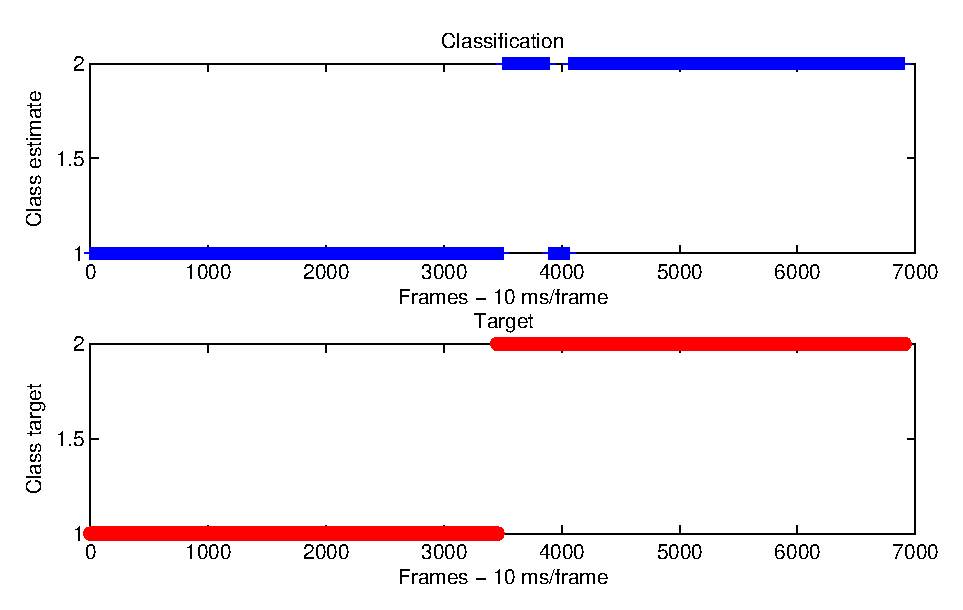
\includegraphics{SVM_1digit_PCA10}
\caption{Results of using SVM classifiers and one digit spoken}
\label{fig:Lin_fig_10}
\end{figure}

\begin{table}[H]                                                    
\centering                                                          
\begin{tabular}{|l|c|c|c|}                                          
\hline                                              
  & Speaker Jacob & Speaker Mose & Precision [\%] \\
\hline                                              
Estimate Jacob & 3454.0 & 211.0 & 94.2 \\           
\hline                                              
Estimate Mose & 0.0 & 3243.0 & 100.0 \\             
\hline                                              
Sensitivity [\%] & 100.0 & 93.9 & 96.9 \\           
\hline                                              
\end{tabular}                                       
\caption{Confusion matrix - 1 digit}                
\label{table:SVM_conf_1}                            
\end{table} 

\subsection{Two digits:}

\subsection{Ten digits:}

\section{Discussion}

% K-means clustering - MANGLER theory and reasons to dump it
\chapter{K-means clustering}
K-means clustering is an unsupervised machine learning algorithm for finding sub populations in unlabelled data.
It has not been applied to this case, but is reviewed for sake of completeness and to help understanding of Gaussian Mixture Models (See chapter \ref{sec:GMM}) 
\section{Theory} 

K-means basically works by iteratively estimating K cluster means and assigning responsibility according to euclidean distance.

\subsection{The K-means algorithm}

\begin{enumerate}

\item
Choose the number, K, of clusters to fit.

\item
Pick K random guesses of mean values $ \mu_j $ or mean vector $ \bm{\mu}_k $ for multi dimensional data.

\item \label{itm:Kmean_Est}
Assign responsibility of all data point by smallest euclidean distance to cluster mean.

\begin{equation}
r_{nk} =
  \begin{cases}
    1 & \text{if } k = 
    	\argmin_j \lVert \mathbf{x}_n - \bm{\mu}_j \rVert^2\\
    0 & \text{otherwise}
  \end{cases} 
\end{equation}

Where $ r_{nk} $ is 1 if cluster $ k $ is responsible for $ \mathbf{x}_n $ 

\item \label{itm:Kmean_Max}
Estimate new cluster means from cluster assignments

\begin{equation}
\bm{\mu}_k = 
\dfrac{\sum_n r_{nk}\mathbf{x}_n}
{\sum_n r_{nk}}
\end{equation}

\item
Repeat from \ref{itm:Kmean_Est}. until stopping criteria is met e.g. no change in cluster assignments or change in cluster means below pre-set threshold. 

\end{enumerate}

\begin{figure}[H]
	\centering
	\begin{subfigure}[H]{0.3\linewidth}
		\includegraphics{Figure9_1a}
		\label{fig:F9.1a}
	\end{subfigure}
	\quad
	\begin{subfigure}[H]{0.3\linewidth}
		\includegraphics{Figure9_1b}
		\label{fig:F9.1b}
	\end{subfigure}
	\quad
	\begin{subfigure}[H]{0.3\linewidth}
		\includegraphics{Figure9_1c}
		\label{fig:F9.1c}
	\end{subfigure}
	
	
	\begin{subfigure}[H]{0.3\linewidth}
		\includegraphics{Figure9_1d}
		\label{fig:F9.1d}
	\end{subfigure}
	\quad
	\begin{subfigure}[H]{0.3\linewidth}
		\includegraphics{Figure9_1e}
		\label{fig:F9.1e}
	\end{subfigure}
	\quad
	\begin{subfigure}[H]{0.3\linewidth}
		\includegraphics{Figure9_1f}
		\label{fig:F9.1f}
	\end{subfigure}
	

	\begin{subfigure}[H]{0.3\linewidth}
		\includegraphics{Figure9_1g}
		\label{fig:F9.1g}
	\end{subfigure}
	\quad
	\begin{subfigure}[H]{0.3\linewidth}
		\includegraphics{Figure9_1h}
		\label{fig:F9.1h}
	\end{subfigure}
	\quad
	\begin{subfigure}[H]{0.3\linewidth}
		\includegraphics{Figure9_1i}
		\label{fig:F9.1i}
	\end{subfigure}
	
	\caption{Four iterations of K-means on the Old Faithful data set}

\end{figure}

\section{Discussion}

In this project K-means could have been used to make a sort of mixture model of each speaker, by fitting a number of clusters to the different unique sounds the individual speaker makes and then for a series of samples evaluating which speaker is most likely to have emitted the sounds.

It has been elected not to try to apply K-means to this project as it does not fit this application very well, as opposed like other more advanced methods like Artificial Neural Networks (Chapter \ref{sec:ANN}) or Gaussian Mixture Models (Chapter \ref{sec:GMM}).
  

% Hidden Markov Models - MANGLER theory and reasons to dump it
\chapter{Hidden Markov Models}
In this project the Hidden Markov models (HMM) is not used on the data.
The reason for this is that the HMM is optimized for recognizing the sequence of the sounds which combines to a word.
HMM is focused on speech recognition and not speaker recognition, which is this project works with.

\section{Theory}   
The HMM is developed to process sequential information in the data, in other models the features have been treated as independent and identical distribution.
When classifying speech from a sequence of data recorded over time, the features tend to be strongly associate with the previous features.
The associated features can be exploited by the Markov model to classify, the model uses join distributions to link the relationship between two or more successive data points $ \left\lbrace \mathbf{x}_1,...,\mathbf{x}_N \right\rbrace  $.
\begin{equation}
p(\mathbf{x}_1,...,\mathbf{x}_N) = 
\prod_{n=2}^{N} 
p(\mathbf{x}_n | \mathbf{x}_1,...,\mathbf{x}_{n-1})
\label{eq:HMM_JD}
\end{equation} 
The right hand-side describes the probability of a transition from one data point to the next.

If the data is noisy, an addition to Markov model can be used, which is called Hidden Markov model.
The HMM uses discrete hidden states $ \left\lbrace \mathbf{z}_1,..., \mathbf{z}_N \right\rbrace  $.
The jointed distributions in the HMM can be formulated so
\begin{equation}
p(\mathbf{X},\mathbf{Z}|\Theta) = 
p(\mathbf{z}_1|\pi)
\left(\prod_{n=2}^{N} p(\mathbf{z}_n|\mathbf{z}_{n-1},\mathbf{A}) \right)
\prod_{m=1}^{N} p(\mathbf{x}_m|\mathbf{z}_m,\phi) 
\label{eq:HMM}
\end{equation}
Where $ \mathbf{X} = \left\lbrace \mathbf{x}_1,...,\mathbf{x}_N \right\rbrace  $, $ \mathbf{Z} = \left\lbrace \mathbf{z}_1,...,\mathbf{z}_N \right\rbrace  $ and $ \Theta = \left\lbrace \pi, \mathbf{A}, \phi \right\rbrace  $ is the models parameters. The parameter $ \pi $, is the initial parameter and \textbf{A} is the transition parameter, which holds the probabilities for transition between each hidden state.
The parameter $ \phi $, is the emission parameter. 

Given a set of data points the goal is to determine the model parameters in the HMM. This can be done by applying an estimation maximization algorithm on the following equation
\begin{equation}
Q(\Theta,\Theta^{\mathtt{old}})=
\sum_{\mathbf{z}}^{} p(\mathbf{X},\mathbf{Z}|\Theta^{\mathtt{old}})
\ln p(\mathbf{X},\mathbf{Z}|\Theta)
\end{equation}
\fxnote{Er det store Theta?}
             


\bibliographystyle{ieeetr}
\renewcommand{\bibname}{Reference Document}
\addcontentsline{toc}{chapter}{2 Reference Document}
\bibliography{10731@post.au.dk-RefList}

\end{document}          
